\documentclass[11pt,letterpaper]{article}

\usepackage[spanish,es-tabla,es-nodecimaldot]{babel}
\usepackage{amsmath}
\usepackage[utf8]{inputenc}
\usepackage[T1]{fontenc}
\usepackage{lmodern}
\usepackage{graphicx}
\usepackage{listings}
\usepackage{anysize} 
\usepackage{fancyhdr}
\usepackage{amsmath}
\usepackage{pdfpages}
\usepackage{graphics}
\usepackage{capt-of}
\usepackage{tabularx}
\usepackage{rotating}
\usepackage{tikz}
\usepackage[colorlinks=true,plainpages=true,citecolor=blue,linkcolor=blue]{hyperref}


\marginsize{2cm}{2cm}{2cm}{2cm}
\pagestyle{fancy}
\fancyhf{Sistemas celulares}
\fancyhead[L]{\footnotesize UPIITA-IPN} 
\fancyhead[R]{\footnotesize 2TV7} 
\fancyfoot[R]{\footnotesize Tarea 2}
\fancyfoot[C]{\thepage}
\fancyfoot[L]{\footnotesize } 

\renewcommand{\footrulewidth}{0.4pt}
\renewcommand{\spanishtablename}{Tabla}
\renewcommand{\labelitemii}{$\star$}
\graphicspath{ {C:/Users/Anselmo/Documents/GitHub/upiita-SistemasCelulares/Tarea2/imagenes} }

\begin{document}
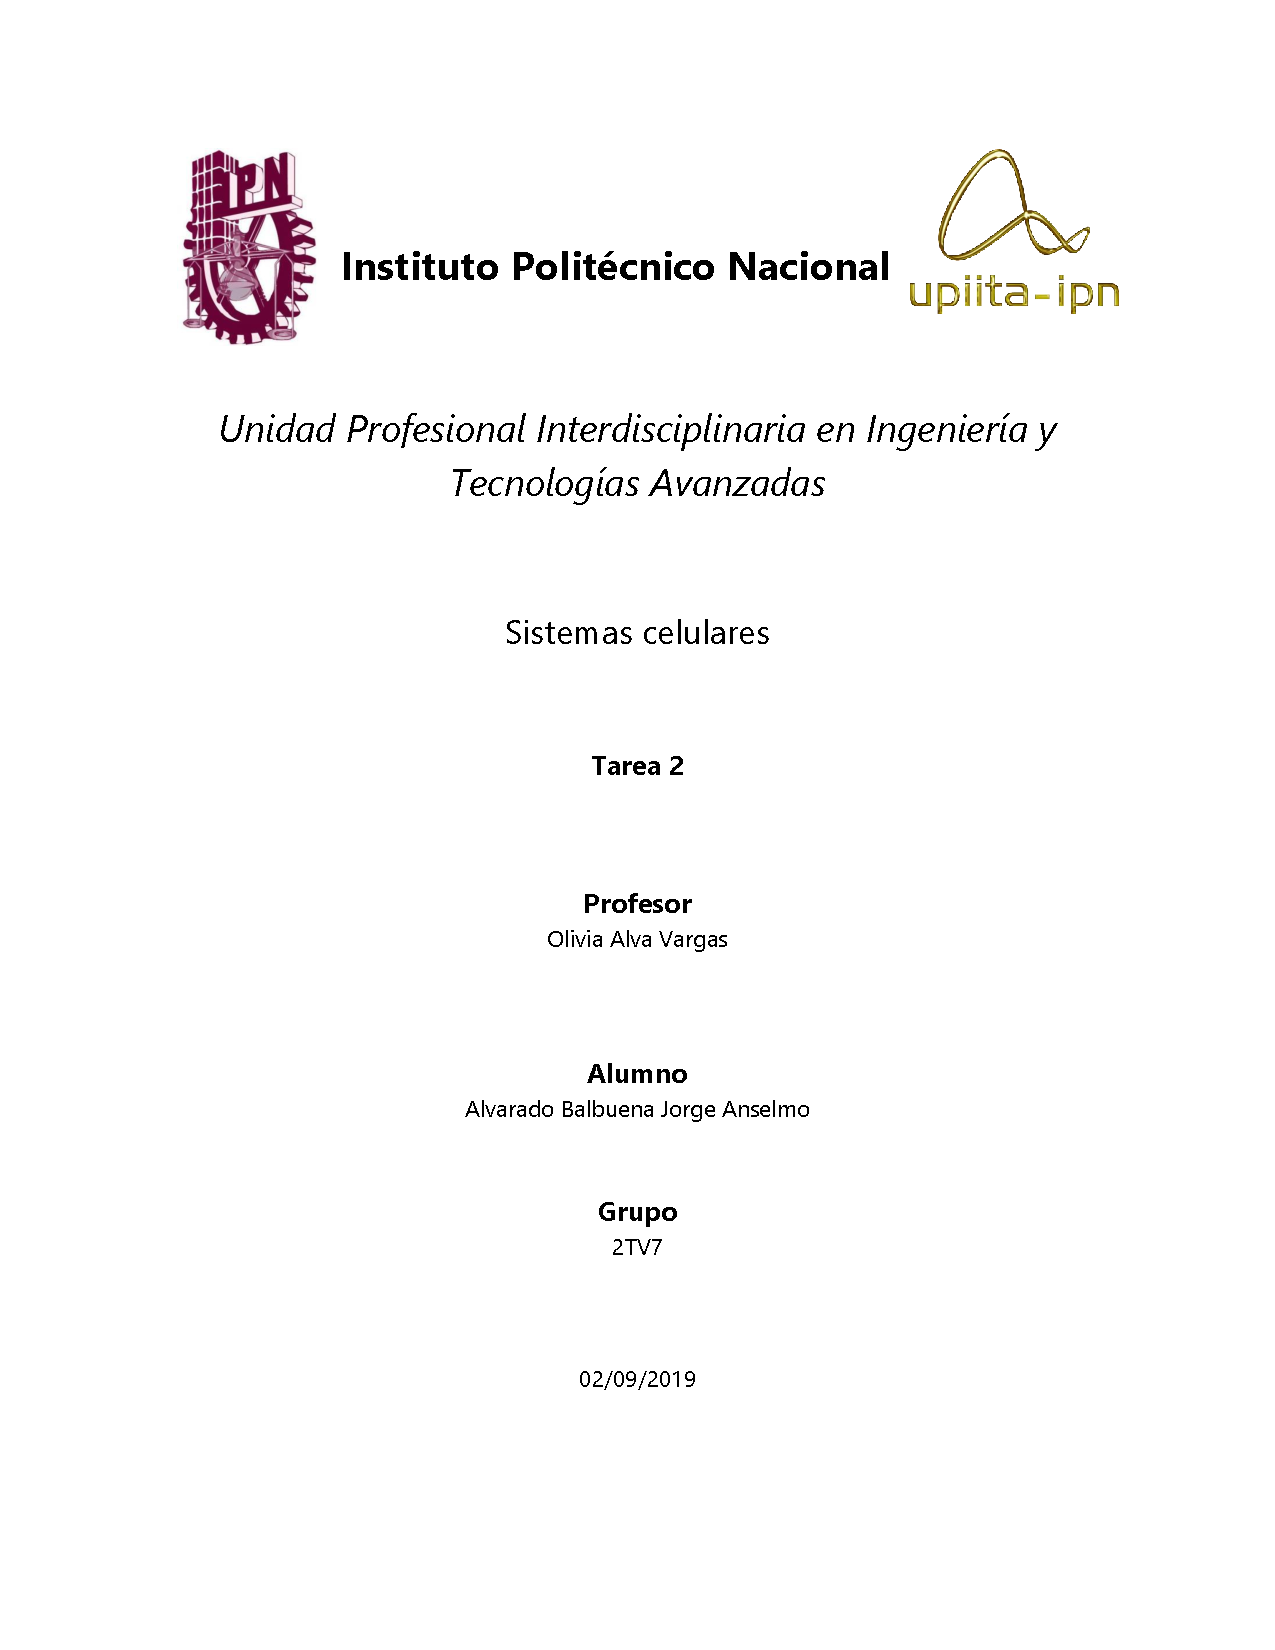
\includepdf[pages={1}]{Portada}

\newpage
\tableofcontents
\listoffigures
\listoftables

\newpage
\section{Área de estudio}
\subsection{Contexto}
Nezahualcóyotl es una ciudad y uno de los 125 municipios del Estado de México. Se localiza 
al oriente de la Ciudad de México y en la región oriente del Estado de México. Posee una 
superficie de 63.74 $km^2$ y una población de 1,109,363 habitantes; cada kilómetro de 
superficie alberga 17,537 personas, la densidad de población más alta del país.
\\ \\
Es uno de los municipios con mayor densidad poblacional. Considerado una ciudad dormitorio 
por su carácter mayoritariamente residencial, en las últimas décadas ha repuntado en su 
capacidad económica, producción de empleos y de impacto socioeconómico a los municipios 
adyacentes. \cite{uno}
\\ \\
\textbf{Datos demográficos}
\begin{itemize}
    \item Coordenadas: 19,24 N 98,59 O.
    \item Superficie: 63.74 $km^2$.
    \item Altitud media: 2220m ASNM.
    \item Población total: 1,228,654 hab.
    \item Densidad poblacional: 175,369 $hab/km^2$
\end{itemize}

\section{Cálculo de reuso de frecuencias para sistema AMPS}
\subsection{Área del patrón de radiación}
De acuerdo con las especifiaciones dadas, el área del cardiode debe ser de 1 $km^2$. Para ello 
se utilizará la siguiente formula.

\begin{equation}
    A=\int_{0}^{\pi} \rho^2 d\theta = \frac{3}{2} a^2 \pi
\end{equation}
\\
Resolviendo para $a$, da un resultado de: 0.212 km.
\begin{figure}[ht]
    \centering
    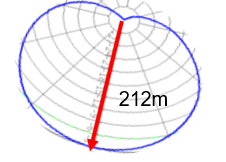
\includegraphics[width=0.3\textwidth]{imagenes/t10.png}
    \caption{Patrón de radiación de acuerdo con el resultado obtenido.}
\end{figure}

\newpage
\section{Distribución de frecuencias}
\begin{figure}[ht]
    \centering
    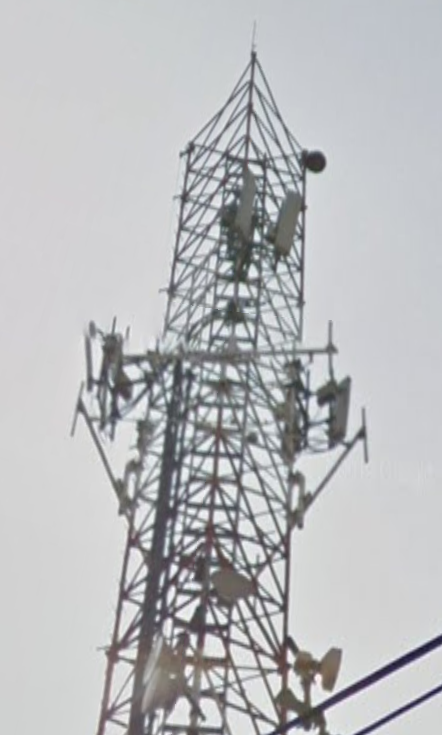
\includegraphics[width=.9\textwidth, angle=90]{imagenes/t11.png}
    \caption{Patrón de radiación de acuerdo con el resultado obtenido.}
\end{figure}

\newpage
\subsection{Distribución de canales en celulas}
\subsubsection{Clúster 1}
\begin{itemize}
    \item Cel 1 (1-95)
    \item Cel 2 (96-191)
    \item Cel 3 (192-287)
    \item Cel 4 (288-383)
    \item Cel 5 (384-479)
    \item Cel 6 (480-575)
    \item Cel 7 (576-671)
\end{itemize}

\subsubsection{Clúster 2}
\begin{itemize}
    \item Cel 1 (1-95)
    \item Cel 2 (96-191)
    \item Cel 3 (192-287)
    \item Cel 4 (288-383)
    \item Cel 5 (384-479)
    \item Cel 6 (480-575)
    \item Cel 7 (576-671)
\end{itemize}

\subsubsection{Clúster 3}
\begin{itemize}
    \item Cel 1 (1-222)
    \item Cel 2 (223-445)
    \item Cel 3 (446-668)
\end{itemize}

\newpage
\subsection{Cálculo de $P_{Rx}$ en áreas vulnerables}
Dado el escenario asignado de la década de los 80s, se eligió un umbral de -75$dB$ para 
permitir la comunicación.
\\ \\
Con la ayuda de la siguiente formula y resolviendo para $b$ se obtendrá la distancia a la 
que este umbral es alcanzado.
\begin{equation}
    P_{Rx}=(\frac{hb*hm}{d^2})^2 (\frac{G_{Tx}*G_{Rx}}{L_0}) P_{Tx}
\end{equation}
Donde:
\begin{itemize}
    \item $P_{Rx}$: -80 dB.
    \item $G_{Tx}$: 0.86 dB.
    \item $G_{Rx}$: 9 dB.
    \item $P_{Tx}$: 0.1 W.
    \item hm: 1.75 m.
\end{itemize}

\subsubsection{Cálculo promedio para primer cluster}
\begin{itemize}
    \item hb: 29 m.
\end{itemize}
\textbf{Resultado: 1115m}

\subsubsection{Cálculo promedio para segundo cluster}
\begin{itemize}
    \item hb: 27 m.
\end{itemize}
\textbf{Resultado: 1080m}

\subsubsection{Cálculo promedio tercer cluster}
\begin{itemize}
    \item hb: 26m.
\end{itemize}
\textbf{Resultado: 1065m}
\\ \\
Estos resultados da un prodemio de distancia $d=1086.6$ m.

\newpage
\section{Eficiencia espectral y trafico}
Con un grado de servicio de \%80 se tiene lo siguiente.
\begin{equation}
    \frac{100-GoS}{100}=0.2
\end{equation}
\\
La población estimada en la decada de lo 80s en el municipio de Nezahualcoyotl:
\begin{equation}
    1228654 \ hab * 0.05 = 61432.7 \ usuarios
\end{equation}
\\
\subsection{Descripción de clústers}
\begin{figure}[ht]
    \centering
    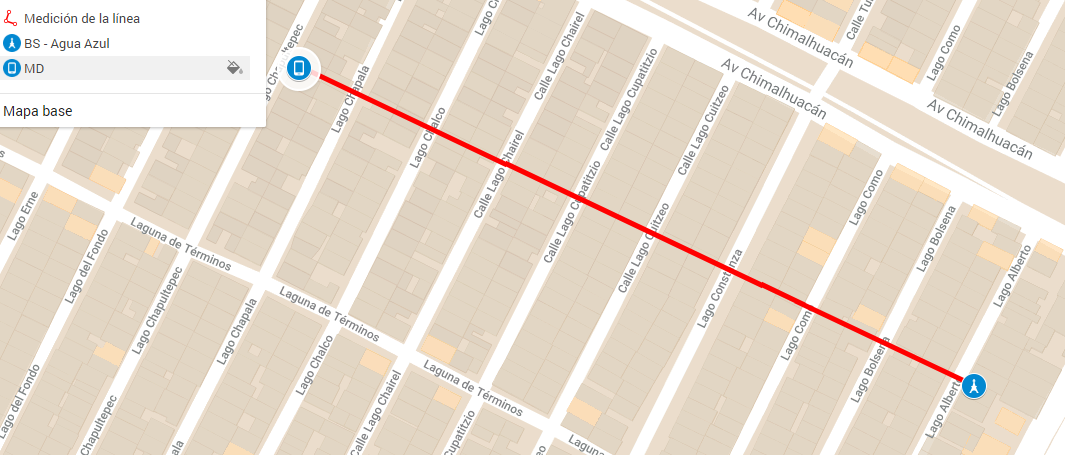
\includegraphics[width=.5\textwidth]{imagenes/t12.png}
    \caption{Clústers.}
\end{figure}

Con la siguiente expresión se calculará la eficiencia expectral.
\begin{equation}
    %\eta=\frac{\frac{\frac{BW_{SIS}}{BW_{CH}}}{N_C}}{BW_{SIS}*Area}
    \eta=\frac{Tráfico \ Erlang}{BW_{SIS}*Area}
\end{equation}
Donde:
\begin{itemize}
    \item Área: 63.74 $km^2$.
    \item $BW_{SIS}=24$ MHz.
    \item $BW_{CH}=30$ MHz.
\end{itemize}

Posteriormente se econtrará los Erlangs de acuerdo con el número de canales que se tienen.
\\ \\
$n=301 => A=371.52 \ Erlnag$
\\ \\
$n_c=2010->A_c=2480.91 \ Erlnag$
\\ \\
Sustituyendo, la eficiencia resulta.
\begin{equation}
    %\eta=\frac{\frac{\frac{BW_{SIS}}{BW_{CH}}}{N_C}}{BW_{SIS}*Area}
    \eta=\frac{2480.91}{24*63.74}=1.621 \ Erlnag/MHz/Km^2
\end{equation}
\\ \\
Ahora, el número de llamadas.
\\ \\
Si A=2480.91 Erlangs y resolviendo para N.
\begin{equation}
    A=\frac{N*\overline{t}}{hp}
\end{equation}
Donde:
\begin{itemize}
    \item $\overline{t}$: Tiempo pormedio de llamada = 180s.
    \item hp: Hora pico de medición = 3600s.
    \item N: Cantidad de llamadas necesarias en función de la población.
\end{itemize}
\begin{equation}
    N=\frac{A*hp}{\overline{t}}=\frac{2480.91*3600}{180}=49618.2
\end{equation}
Por último, se obtiene la relación de número de llamadas por población.
\begin{equation}
    \frac{N}{p(80s)}=0.807 \ [\frac{llamada}{hora}]
\end{equation}

\newpage
\section{Conclusiones}
Revisando los resultados obtenidos se puede observar que el diseño propuesto no cumple los 
requqerimientos para que los usuarios de la red realicen una llamada con exito. Revisando el 
diseño de la red, se puede sugerir un mayor número de celulas más cerca entre si. Es importante 
recordar que el municipio de Nezahualcoyotl es una de la regiones con mayor densidad poblacional 
del país. Se debe considerar este dato, ya que cada célula debe de dar servicio a un gran número 
de usuarios. 

\begin{thebibliography}{20}
    \bibitem{uno} 
    $https://es.wikipedia.org/wiki/Nezahualcoyotl$

\end{thebibliography}

\end{document}